\documentclass{beamer}

\usepackage[utf8]{inputenc}
\usepackage{graphicx}

%Information to be included in the title page:
\title{Numerical Methods with Python}
%\author{Anonymous}
%\institute{Overleaf}
\date{}



\begin{document}
	
	\frame{\titlepage}
	
	\begin{frame}
		\frametitle{Numerical Integration}
		Problem Statement:
		\begin{itemize}
			\item <1->Given some known function $f(x)$, we wish to calculate the definite integral from $x_1$ to $x_2$
			\item <2-> Example: $p(t)=p_0+\int_{t_i}^{t_f}F(t)dt$
			\begin{itemize}
				\item Given the function $F(t)$ and the initial momentum $p_0$, we can calculate $p(t)$
			\end{itemize}
			\item <3-> Example: $W=\int_{x_i}^{x_f}F_x(x)dx$
		\end{itemize}
	\end{frame}

	\begin{frame}
		\frametitle{Numerical Integration}
		What \textit{is} an integral?\\
		Question: if $y(x)$ is a curve describing the boundary of some shape, what does $\int_{x_{min}}^{x_{max}}y(x)dx$ represent?
		\begin{itemize}
			\item <2-> It is just the \textbf{area under the curve}
		\end{itemize}
	\end{frame}

	\begin{frame}{Example: a triangle}
		
	\end{frame}

	\begin{frame}{Numerical Integration}
		Not all functions are so easy...
		\begin{center}
		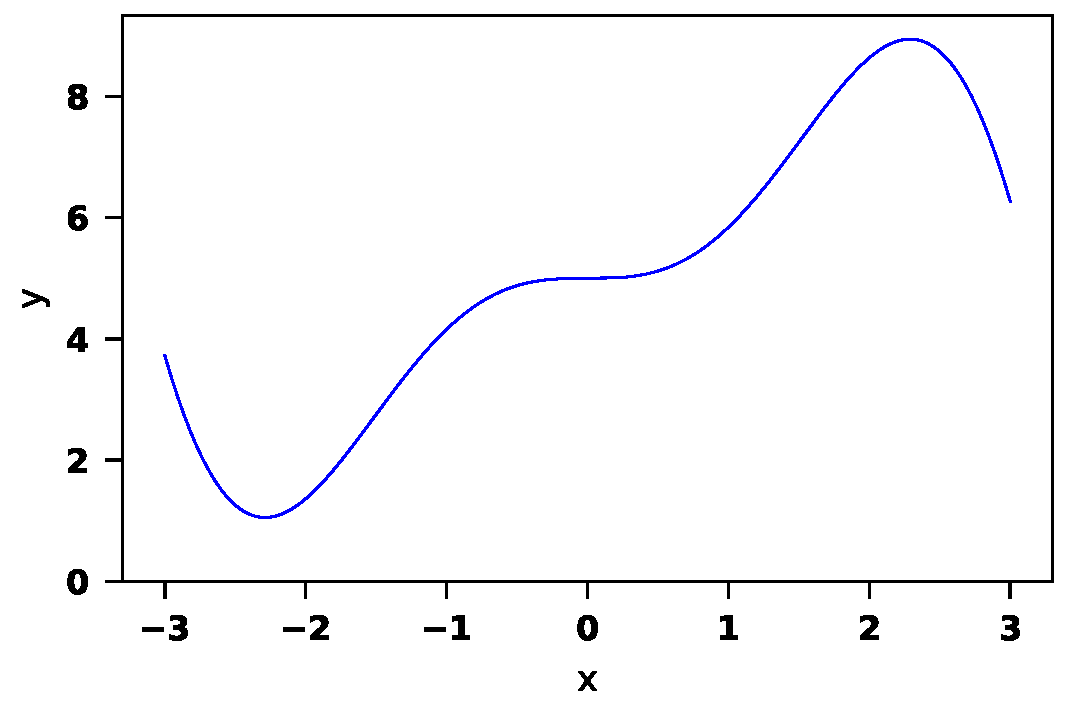
\includegraphics[width=8cm]{complicated_function.pdf}
		\end{center}
	\end{frame}


	\begin{frame}
		\frametitle{Our Approach}
		We don't know the area of this complicated function\\
		We \textit{do} know the area of a rectangle!
		\begin{center}
			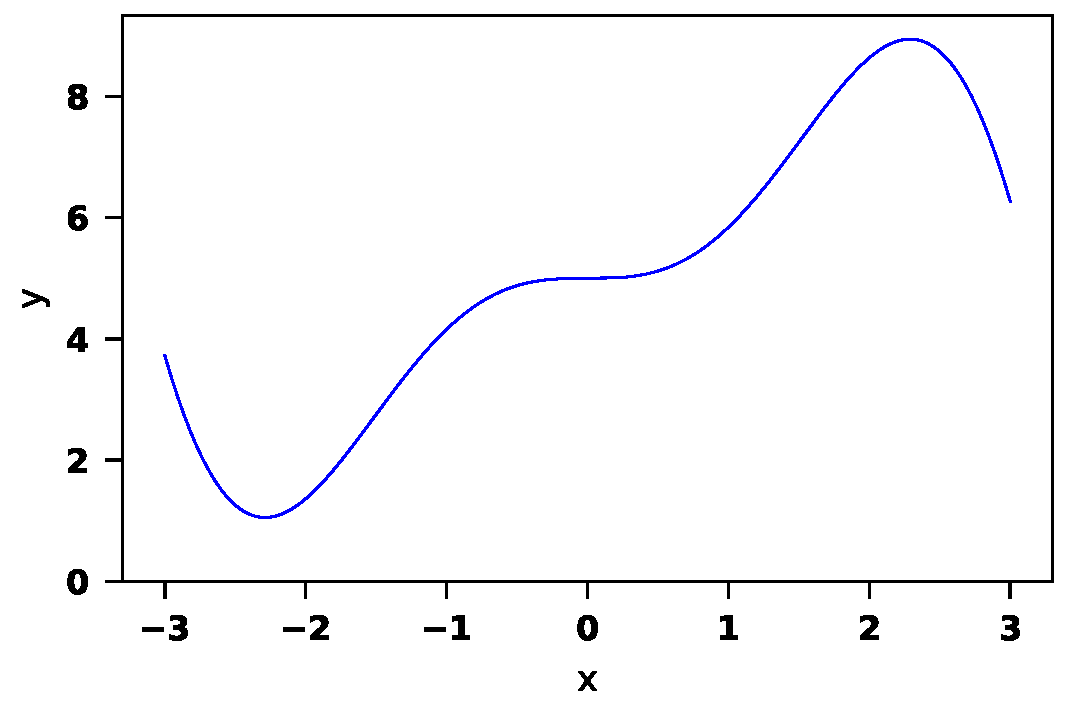
\includegraphics[width=8cm]{complicated_function.pdf}
		\end{center}
	\end{frame}

	\begin{frame}
	\frametitle{Our Approach}
	We don't know the area of this complicated function\\
	We \textit{do} know the area of a rectangle!\\
	\begin{itemize}
		\item 	We can divide the area under the curve into a bunch of tiny rectangles, then add the total area of all of the rectangles
	\end{itemize}
	\begin{center}
		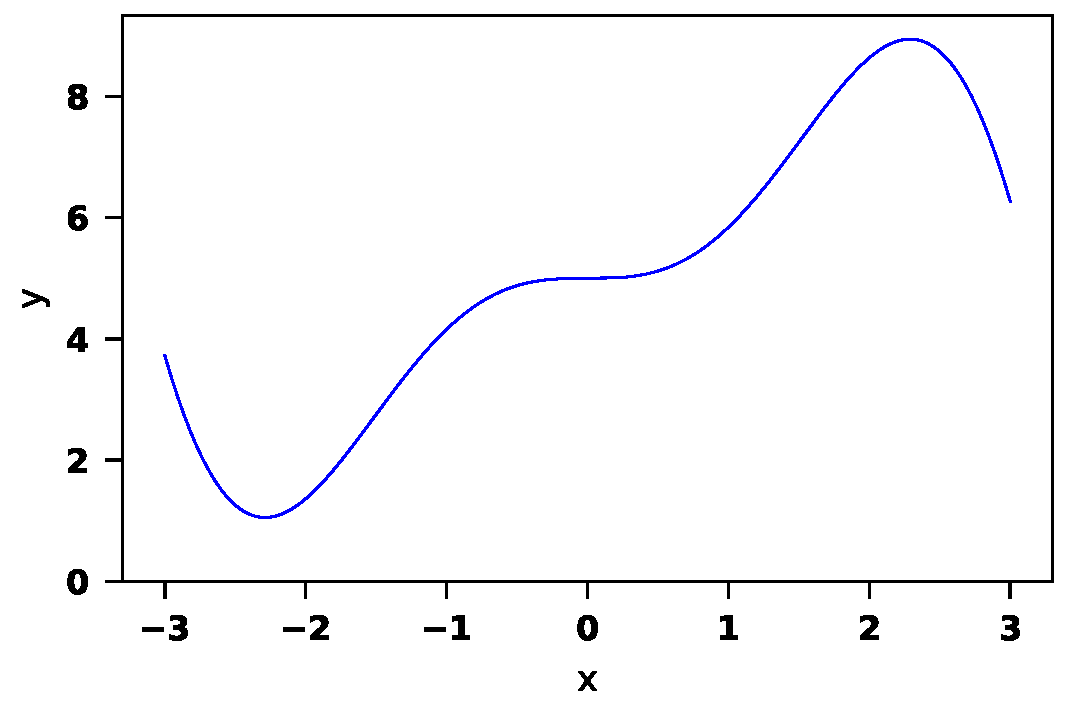
\includegraphics[width=8cm]{complicated_function.pdf}
	\end{center}
	\end{frame}


	\begin{frame}
	\frametitle{Our Approach}
	We don't know the area of this complicated function\\
	We \textit{do} know the area of a rectangle!\\
	\begin{itemize}
		\item 	We can divide the area under the curve into a bunch of tiny rectangles, then add the total area of all of the rectangles
		\item $\int_{-1}^{2}y(x)dx\approx$
	\end{itemize}
	\begin{center}
		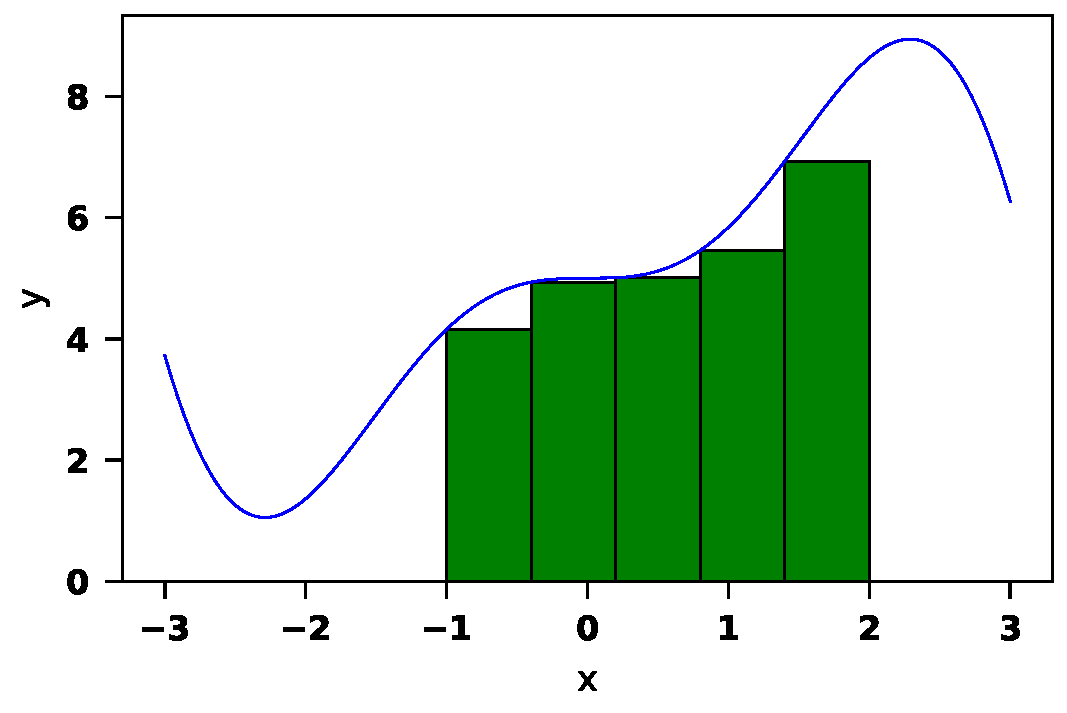
\includegraphics[width=8cm]{reimann_1.pdf}
	\end{center}
	\end{frame}


	\begin{frame}
	\frametitle{Our Approach}
	Each rectangle has a height $h=y(x)$ and a constant width $w=\Delta x$\\
	The area of each rectangle is $h\cdot w$
	\begin{center}
		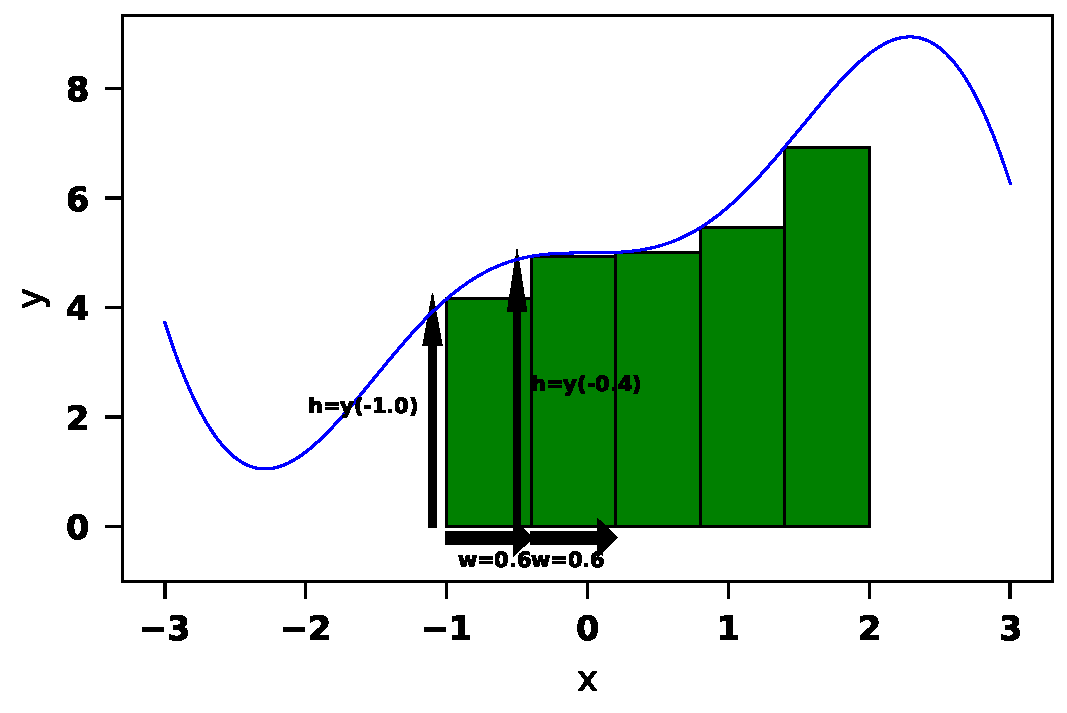
\includegraphics[width=8cm]{reimann_2.pdf}
	\end{center}
	\end{frame}


	\begin{frame}
	\frametitle{Our Approach}
	More generally:
	\begin{center}
		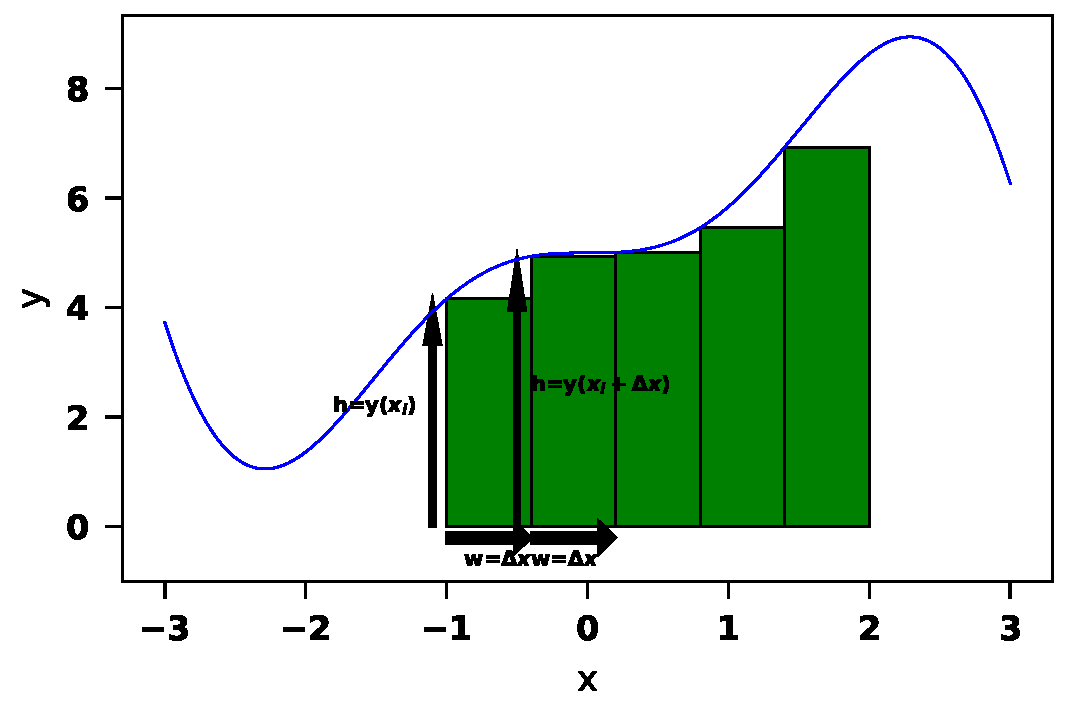
\includegraphics[width=8cm]{reimann_3.pdf}
	\end{center}
	\end{frame}

	\begin{frame}
	\frametitle{Our Approach}
	More generally:
	\begin{equation*}
		\int_{x_i}^{x_f}y(x)dx\approxeq \sum_{k=0}^{n-1}y(x_i+k\Delta x)\cdot\Delta x
	\end{equation*}
	This is called a \textbf{Riemann sum}
	\end{frame}

	\begin{frame}
	\frametitle{Our Approach}
	We can easily code this!
	\begin{enumerate}
		\item Write a function to calculate $y(x)$
		\item Given $x_i$, $x_f$, and $n$, find $\Delta x$
		\item Loop from $k=0$ to $k=n-1$, and sum the quantity $y(x_i+k\Delta x)\cdot \Delta x$
	\end{enumerate}
	\end{frame}

	\begin{frame}
		\href{https://upload.wikimedia.org/wikipedia/commons/1/19/Riemann_sum_\%28leftbox\%29.gif}{https://upload.wikimedia.org/wikipedia/commons/1/19/Riemann\_sum\_\%28leftbox\%29.gif}
	\end{frame}

	\begin{frame}
	\frametitle{Example}
	Integrate $y(x)=2x$ from 0 to 3
	\end{frame}


	\begin{frame}
	\frametitle{Example}
	Integrate $y(x)=e^{-x^2}$ from -1 to 1
	\end{frame}

	\begin{frame}
	\frametitle{Example}
	What if we don't know the functional form of $y(x)$ but we have a set of $(x,y)$ points?
	\end{frame}


	\begin{frame}
		\frametitle{Example}
		Variable acceleration\\
		A certain car has a transmission which enables it to supply a variable force to accelerate the car as a function of time:
		\begin{equation*}
			F(t)=5000\ \mathrm{N} \times (1-e^{-0.2t^3-t^2})
		\end{equation*}
		\begin{center}
			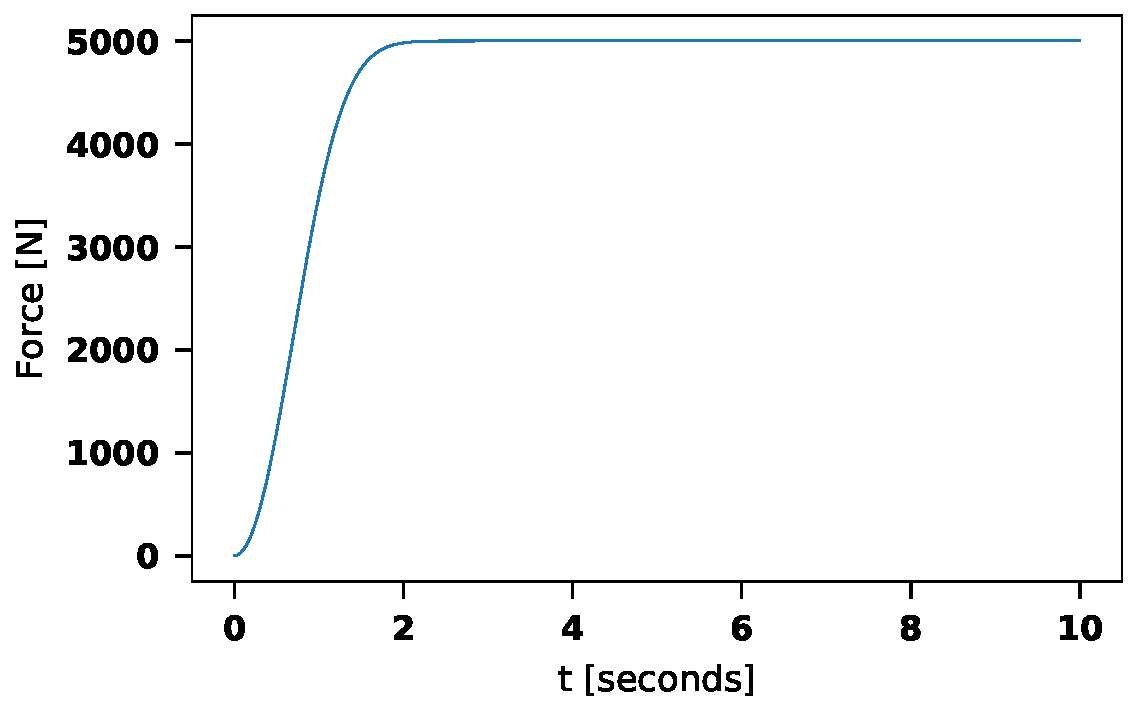
\includegraphics[width=8cm]{variable_force.pdf}
		\end{center}
		Starting from rest, what speed is the 1100 kg car able to travel at after 8 seconds?
	\end{frame}
	\begin{frame}
		\frametitle{Uncertainty of Riemann Estimate}
		This is only an approximation!\\
		The integral
		\begin{equation*}
				I=\int_{x_i}^{x_f}y(x)dx
		\end{equation*}
		has an \textit{exact} answer.\\
		If we knew what it was, we wouldn't need to approximate it!\\
		We are \textit{approximating} this result by:
		\begin{equation*}
			A=\sum_{k=0}^{n-1}y(x_i+k\Delta x)\cdot\Delta x\approxeq\int_{x_i}^{x_f}y(x)dx
		\end{equation*}
	\end{frame}


	\begin{frame}
	\frametitle{Uncertainty of Riemann Estimate}
	\begin{equation*}
		I=\int_{x_i}^{x_f}y(x)dx
	\end{equation*}
	\begin{equation*}
		A=\sum_{k=0}^{n-1}y(x_i+k\Delta x)\cdot\Delta x\approxeq\int_{x_i}^{x_f}y(x)dx
	\end{equation*}
	In general, $A$ and $I$ will not be the same.\\
	We don't know the exact answer $I$, but we \textit{can} estimate how close our estimate $A$ guaranteed to be to it
	\end{frame}


	\begin{frame}
	\frametitle{Uncertainty of Riemann Estimate}
	We have seen that using a larger number of rectangles $n$ results in a more accurate estimate
	\begin{center}
		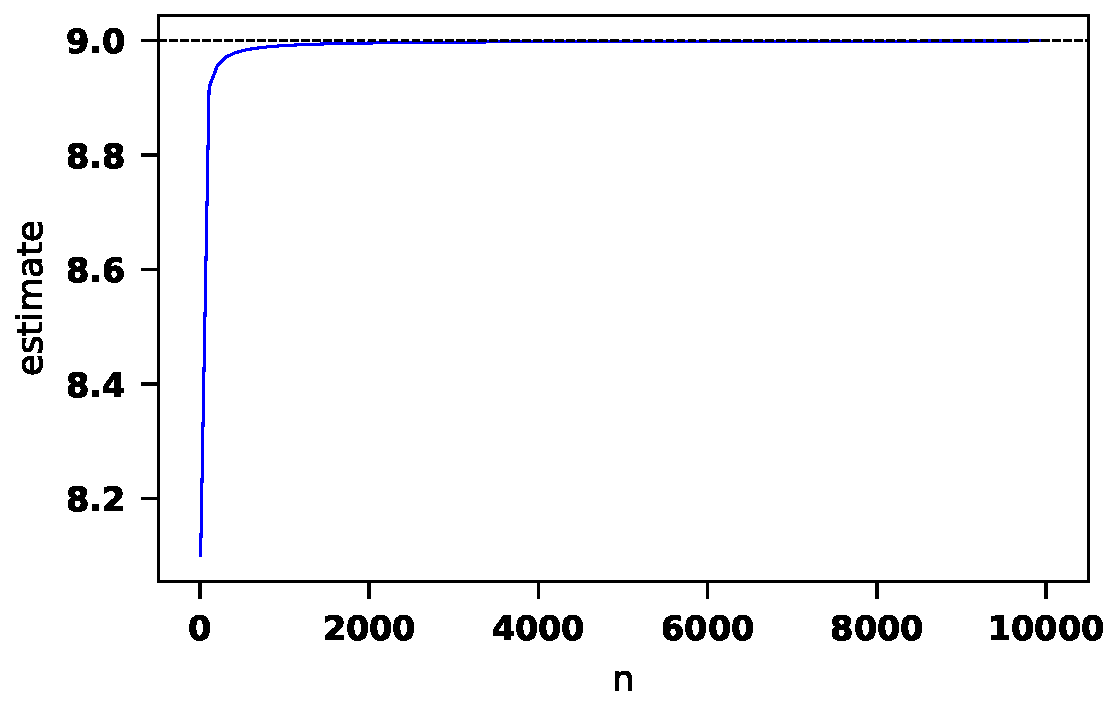
\includegraphics[width=8cm]{error1.pdf}
	\end{center}
	\end{frame}


	\begin{frame}
	\frametitle{Uncertainty of Riemann Estimate}
	In fact, the error of our estimate seems to decrease like $1/n$
	\begin{center}
		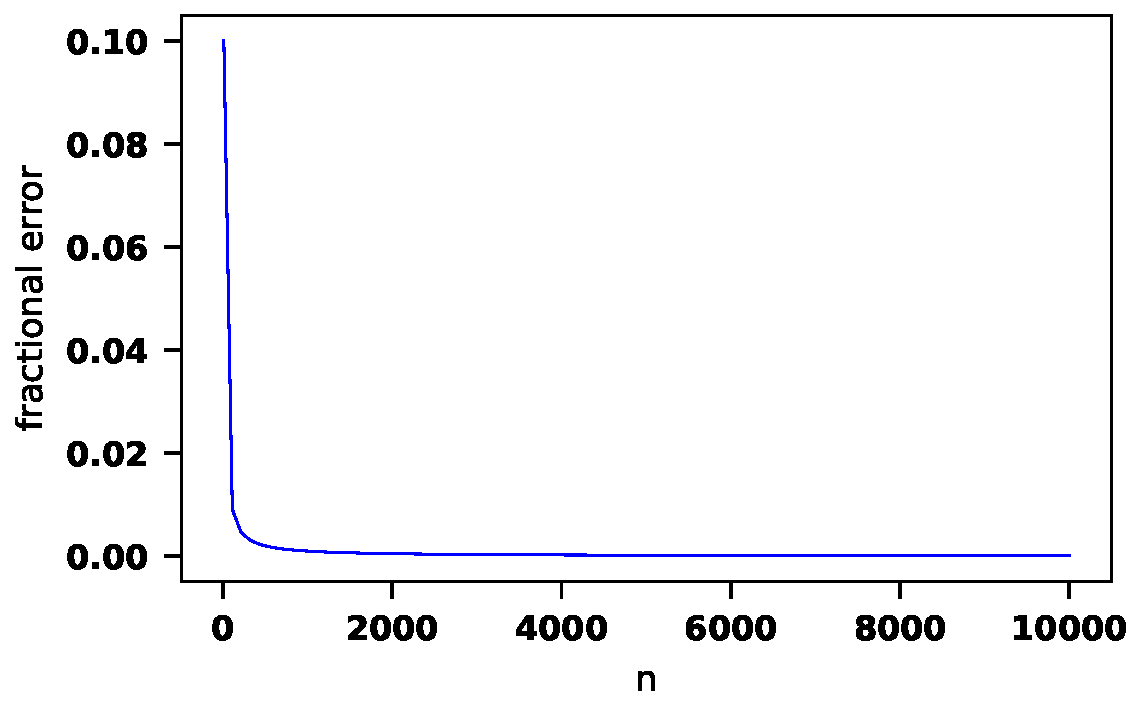
\includegraphics[width=8cm]{error2.pdf}
	\end{center}
	\end{frame}
	
	\begin{frame}
		\frametitle{Uncertainty of Riemann Estimate}
		Let's see if we can quantify the error in our Riemann sum estimate without knowing the true value\\
		\textbf{This is very important!}
		\begin{center}
			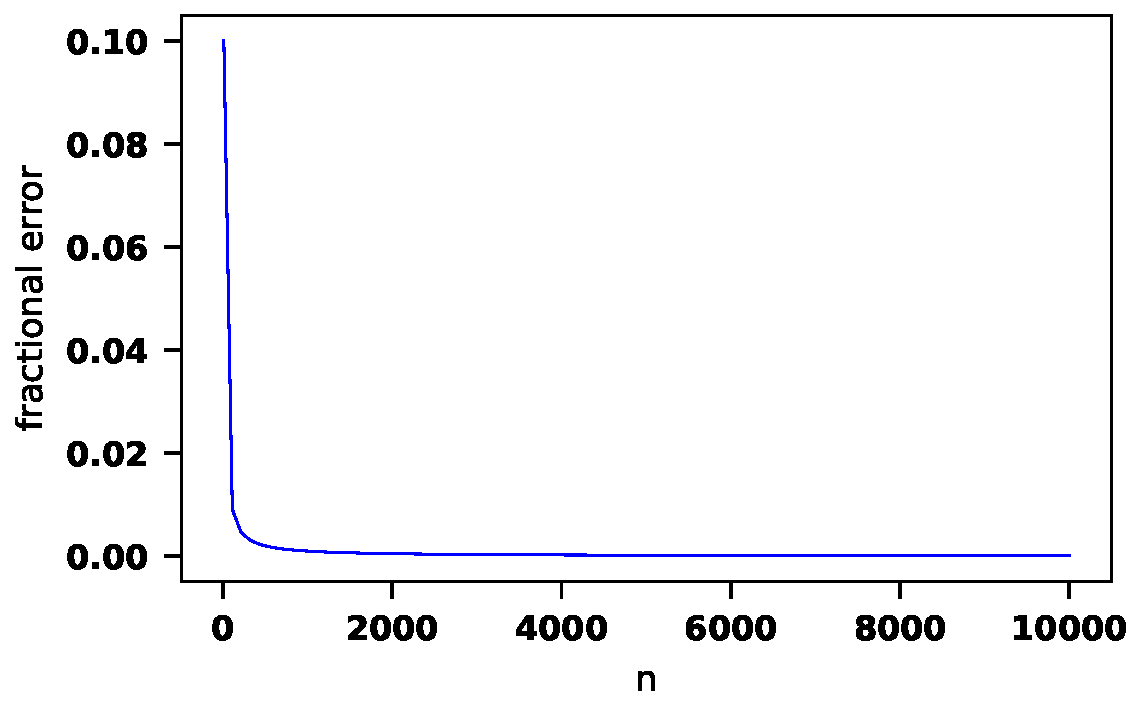
\includegraphics[width=8cm]{error2.pdf}
		\end{center}
	\end{frame}

	\begin{frame}
		\frametitle{Why Estimating Uncertainty is Important}
		As a scientist/engineer, you will be using computer programs to make predictions\\
		\textbf{Your prediction is completely useless unless you know how precise it is!}\\
		If you are asked to calculate how much weight a cable can bear and your program approximates the answer to be 3500 N. 
		\begin{itemize}
			\item We know this answer is probably not the exactly correct value
			\item The correct way to report this result is not ``the cable can hold 3500 N'' but rather ``The true strength of the cable lies somewhere in the range of 3400 N and 3600 N''
			\begin{itemize}
				\item <2-> ``I estimate the strength of the cable to be 3500 N, with a precision of 100 N''
			\end{itemize}
		\end{itemize}
	\end{frame}


	\begin{frame}
	\frametitle{Why Estimating Uncertainty is Important}
	In this case, you probably wouldn't want to hang anything more than 3400 N from the cable
	\begin{itemize}
		\item Even though your estimate is 3500 N, the \textit{true} value could be as low as 3400 N
		\item <2-> If you didn't estimate the uncertainty of your measurement, you would never know this. You would suspend a 3500 N load, and the cable could snap.
	\end{itemize}
	\end{frame}

	\begin{frame}
	\frametitle{Why Estimating Uncertainty is Important}
	In this case, you probably wouldn't want to hang anything more than 3400 N from the cable
	\begin{itemize}
		\item Even though your estimate is 3500 N, the \textit{true} value could be as low as 3400 N
		\item If you didn't estimate the uncertainty of your measurement, you would never know this. You would suspend a 3500 N load, and the cable could snap.
	\end{itemize}
	Any measurement or numerical approximation consists of both a value and an associated uncertainty
	\end{frame}

	\begin{frame}
		\frametitle{Estimating the Uncertainty of a Riemann Sum}
		
	\end{frame}


	\begin{frame}
	\frametitle{Estimating the Uncertainty of a Riemann Sum}
	The absolute error is bounded such that:
	\begin{equation*}
		|E|\leq\frac{1}{2}\frac{M(x_f-x_i)^2}{n}
	\end{equation*}	
	Where:
	\begin{equation*}
		M = \mathrm{max}\left(|y'(x)|, x_i\leq x\leq x_f\right)
	\end{equation*}
	\end{frame}
	
	
	\begin{frame}
	\frametitle{Estimating the Uncertainty of a Riemann Sum}
	$|E|$ is the \textbf{maximum possible} error on our estimate
	\begin{itemize}
		\item We \textit{could} be closer to the actual value
		\item We are \textit{guaranteed} to be within $|E|$ of it
	\end{itemize}
	\end{frame}

	\begin{frame}
	\frametitle{Estimating the Uncertainty of a Riemann Sum}
	$|E|$ is the \textbf{maximum possible} error on our estimate
	\begin{itemize}
		\item We \textit{could} be closer to the actual value
		\item We are \textit{guaranteed} to be within $|E|$ of it
	\end{itemize}
	If $A_{est}$ is our estimate, and $A_{true}$ is the exact result, then:
	\begin{equation*}
		A_{est}-|E|\leq A_{true}\leq A_{est} + |E|
	\end{equation*}
	\end{frame}


	\begin{frame}
	\frametitle{Estimating the Uncertainty of a Riemann Sum}
	Let's modify our code to include the uncertainty along with our actual estimate
	\end{frame}




	\begin{frame}
	\frametitle{Example}
	Variable acceleration\\
	A certain car has a transmission which enables it to supply a variable force to accelerate the car as a function of time:
	\begin{equation*}
		F(t)=5000\ \mathrm{N} \times (1-e^{-0.2t^3-t^2})
	\end{equation*}
	\begin{center}
		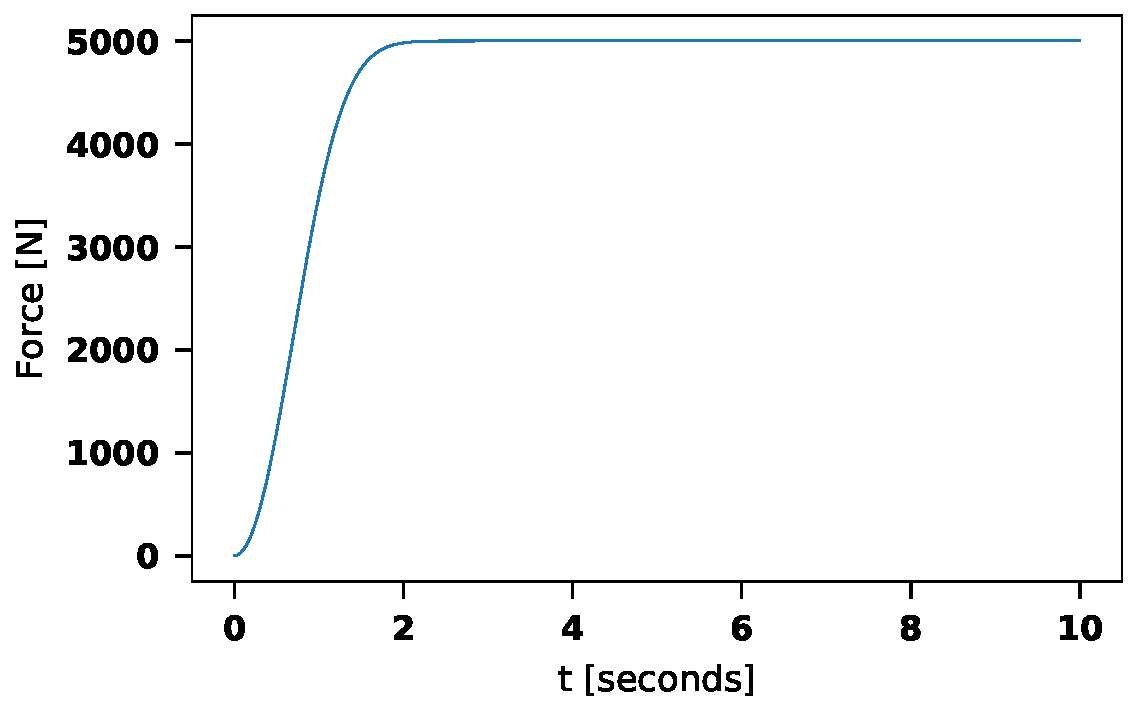
\includegraphics[width=8cm]{variable_force.pdf}
	\end{center}
	Starting from rest, what speed is the 1100 kg car able to travel at after 8 seconds?
\end{frame}

	\begin{frame}
		\frametitle{Improving the approximation}
		We have seen that by using more and more rectangles we can get a better estimate
		\begin{itemize}
			\item <2-> Is there a more efficient way? (A way that would give a closer estimate with the same number of rectangles?)
		\end{itemize}
	\end{frame}

\begin{frame}
	\frametitle{The Midpoint Riemann Sum}
	\begin{center}
		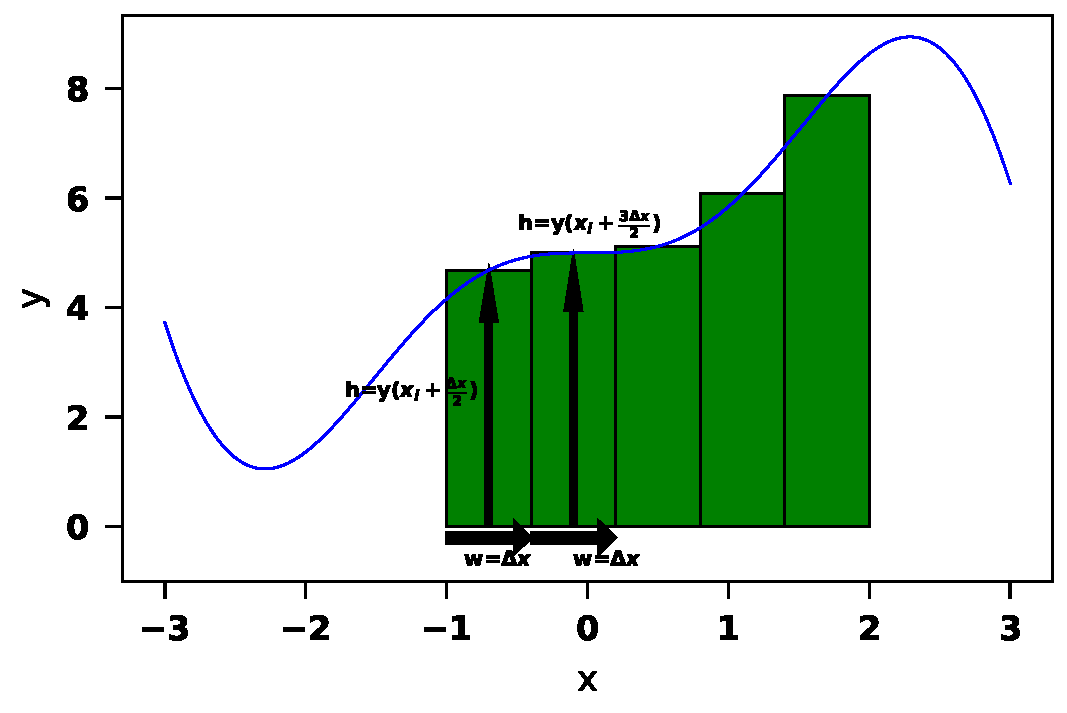
\includegraphics[width=8cm]{reimann_4.pdf}
	\end{center}
\end{frame}

\begin{frame}
	\frametitle{Uncertainty of midpoint method}
	I won't derive this result like the last one, I'll just give you the formula:
	\begin{equation*}
		|E|\leq\frac{1}{24}\frac{M_2(x_f-x_i)^3}{n^2}
	\end{equation*}
	Where $M_2$ is the maximum value of the \textit{second} derivative
\begin{equation*}
	M_2 = \mathrm{max}\left(|y''(x)|, x_i\leq x\leq x_f\right)
\end{equation*}
\end{frame}
\begin{frame}
	\frametitle{Midpoint Riemann vs Left Riemann}
	\begin{center}
		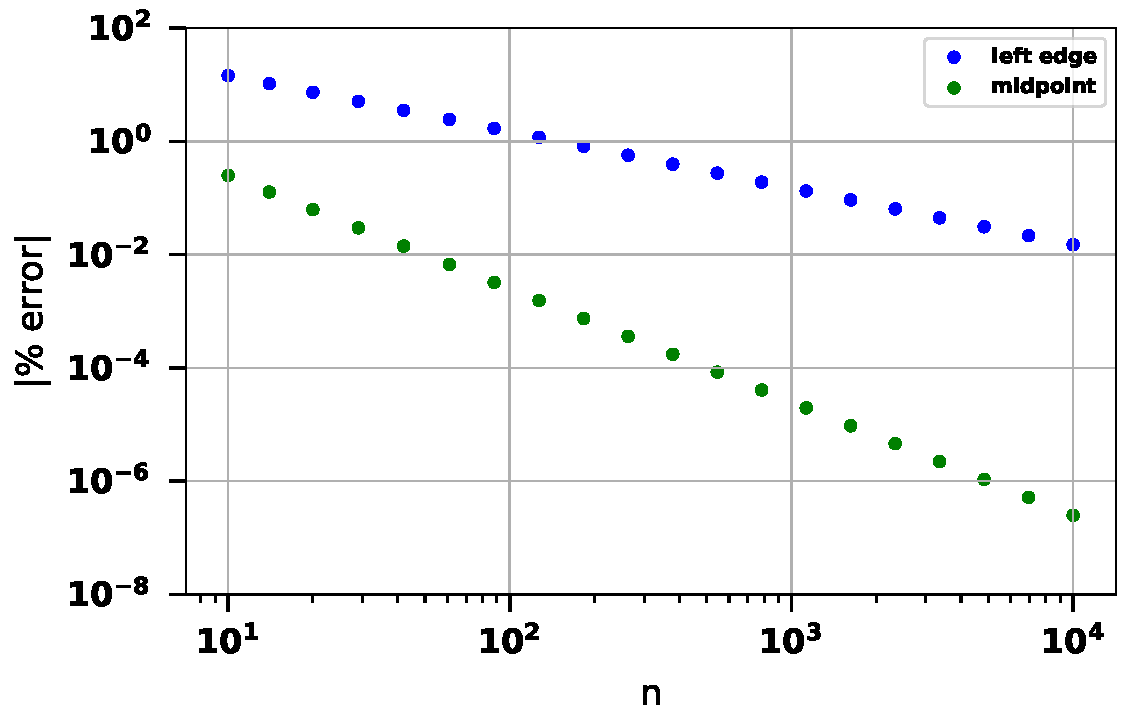
\includegraphics[width=10cm]{left_vs_mid.pdf}
	\end{center}
\end{frame}
\end{document}